\documentclass{article}
\usepackage[utf8]{inputenc}
\usepackage{listings}
\usepackage{amsmath, amssymb}

\title{IBM Quantum Experience Review}
\author{Boettner, Neumann, Gopalan}
\date{May 2020}

\usepackage{xcolor}
\usepackage{graphicx}

\definecolor{codegreen}{rgb}{0,0.6,0}
\definecolor{codegray}{rgb}{0.5,0.5,0.5}
\definecolor{codepurple}{rgb}{0.58,0,0.82}

\lstdefinestyle{qasm}{
    commentstyle=\color{codegreen},
    keywordstyle=\color{magenta},
    numberstyle=\tiny\color{codegray},
    stringstyle=\color{codepurple},
    basicstyle=\ttfamily\footnotesize,
    breakatwhitespace=false,         
    breaklines=true,                 
    captionpos=b,                    
    keepspaces=true,                 
    numbers=left,                    
    numbersep=5pt,                  
    tabsize=2
}

\lstset{style=qasm}
\newcommand{\url}{\footnote{https://quantum-computing.ibm.com/docs/circ-comp/q-gate}} % too long for body
\newcommand{\qasm}{\footnote{https://github.com/Qiskit/openqasm}}
\newcommand{\ibm}{\footnote{https://thequantumdaily.com/2020/01/30/getting-real-time-information-on-ibm-quantum-devices/}}
\begin{document}

\maketitle

\section{The IBM Q System One}
    
    \begin{figure}[h!]
        \centering
        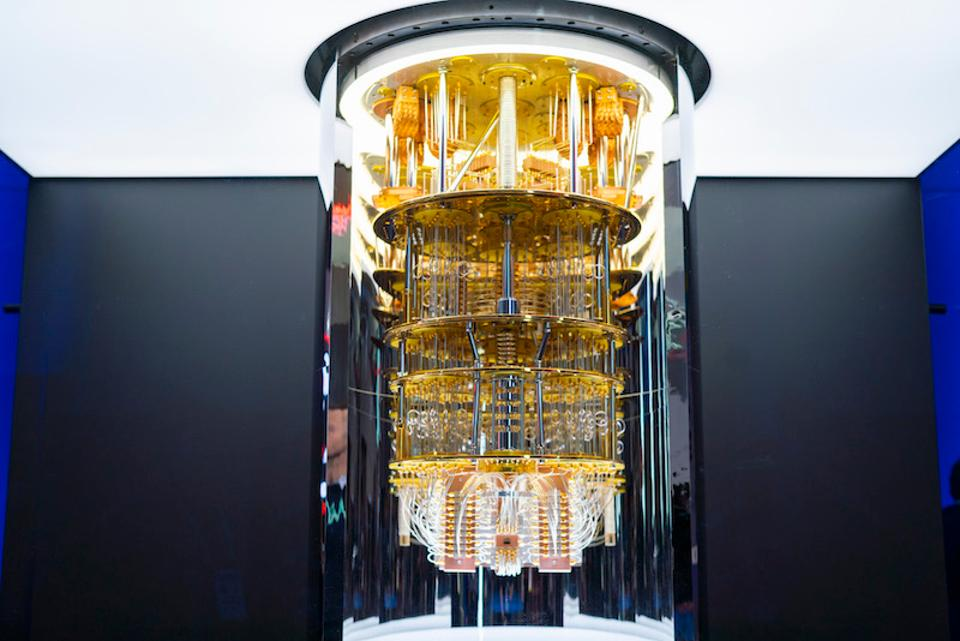
\includegraphics[width=\linewidth]{Circuits/ibm-q.jpg}
        \caption{The IBM Q System One quantum computer}
    \end{figure}
    
    \noindent
    All computing systems rely on a fundamental ability to store and manipulate information. Classical computers manipulate individual bits, which store information as binary 0 and 1 states. Quantum computers, on the other hand, leverage quantum mechanical phenomena to manipulate information. To do this, they rely on quantum bits, or qubits, which are unit vectors in $\mathbb{C}^2$. Storing and manipulating data in the form of qubits leads to more information, which allows for several fast and efficient algorithms for tasks that are significantly harder to solve on a classical computer.
    \\
    \smallskip
    \\
    The history of quantum computing research goes all the way back to 1927 and each result marked a new piece of the puzzle. In October 2017, a significant mathematical result was published in the paper “Quantum Advantage with Shallow Circuits” (Bravyi et al. 2018), which guided the development of algorithms for quantum computing. The significance of this algorithm was that unlike Shor’s algorithm, it proved that a quantum computer can always solve certain problems in a fixed number of steps, no matter the increased input. A classical computer, on the other hand,  would require an increased number of steps as the input increases for the same problems. This made the Quantum Advantage algorithm a solid and necessary brick in the foundation of quantum computing.
    \\
    \smallskip
    \\
    Building on this foundation, in 2019 IBM Quantum designed and built the world’s first integrated quantum computing system for commercial use: IBM Q System One\ibm\,in order to make quantum computers more reliable and stable. IBM Q System One enabled universal approximate superconducting quantum computers to operate beyond the confines of the research lab and is available online for free. In this paper, we recreate circuits to experiment with the Grover’s Search algorithm and the Deutsch-Josza algorithm, and describe both our results as well as what we learned during the process.


\section{Theory}
    \subsection{Deutsch-Jozsa algorithm}
    
    The Deutsch-Jozsa algorithm was the first to show a separation between the quantum and classical difficulty of a problem. Formally, it is defined as follows: Consider a function $f(x)$ that takes as input $n$-bit strings $x$ and returns 0  or 1. Suppose we are promised that $f(x)$ is either a \emph{constant} function that takes the same value $c \in {0,1}$ on all inputs $x$, or a \emph{balanced} function that takes each value 0 and 1 on exactly half of the inputs. \textbf{The goal is to decide whether $f$ is constant or balanced by making as few function evaluations as possible}. 
    \\
    \smallskip
    \\
    
    \subsection{Grover Search algorithm}
    
        
    
    
    
\section{Coding in IBM Q}
    \textbf{IBM Q} was designed to make it as simple as possible to compute the outcome of Quantum circuits. By using a cloud-based compute model and simple data encoding IBM Q allows users to click and drag gates into a circuit, view the encoding of that circuit in the \textbf{QASM} language\qasm, and see the result of running that Quantum circuit on one of IBM's servers. This process is highly documented and user friendly.IBM Q is a cloud-based processing engine for QASM encoded circuits and the IBM quantum experience adds a simple diagram composer to tie everything together. This platform allows a user to compose quantum circuits and test the result on different qubits. This section will outline how to use this platform to make and test quantum circuits and will provide some simple examples of the interface.
    
    \subsection{Diagram Composer}
        The IBM Q circuit composer allows a user to work with the code and a drag and drop interface side by side. This both helps a user learn how to use QASM and make tweaks to the code or visual easily. 
        (what is the composer and how does it work) click $\rightarrow$ drag
        \begin{figure}
            \centering
            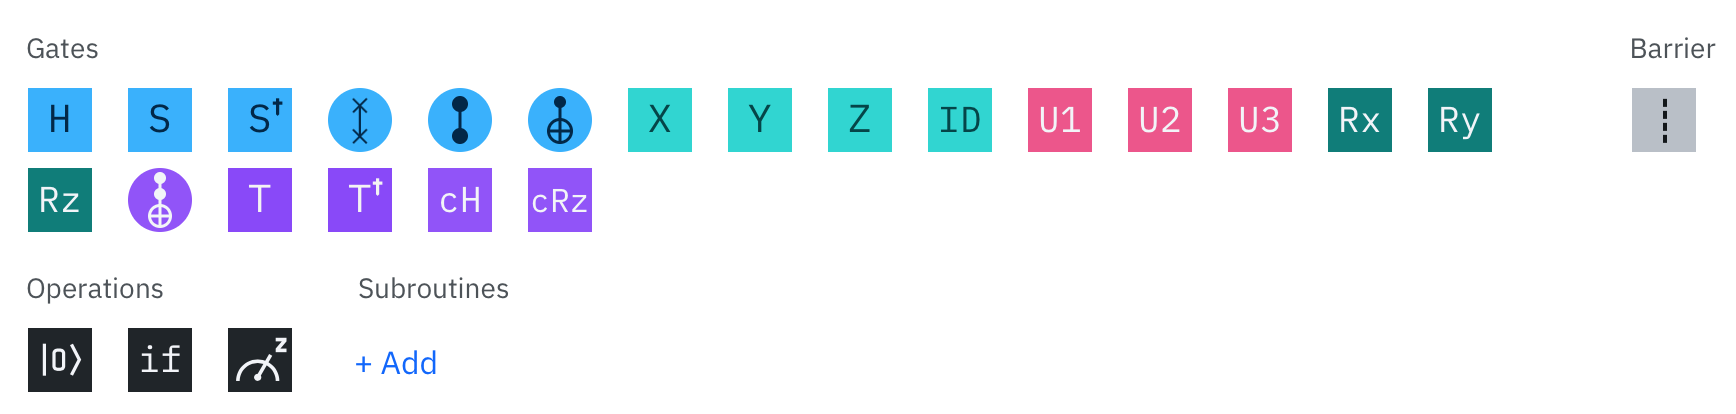
\includegraphics[width=\linewidth]{Circuits/gates.png}
            \caption{Gates in IDM Q}
        \end{figure}
        
    \subsection{Encoding}
        Circuit encoding in IBM Q is pretty simple. This software uses the QASM language developed by IBM in 2017. The QASM language uses arrays to represent qubit input states. In QASM gates are encoded by a short letter or letters\url these gate names are followed by the lines they work on (separated by commas). This encoding allows for complicated gates to be simplified to as few characters as possible. The IBM Q experience software also uses this encoding to send a users circuit to the server they want to analyze it with.
        \\
         \smallskip
        \\
        Encoding a circuit into a small file is a crucial element of IBM Q as all of the computation is done on remote servers. Encoding a circuit into a simple text file allows a user to take advantage of IBM's cloud computing while minimizing the data transmitted between server and client. This allows IBM Q to process multiple circuits at once and allows users to use a server more convenient to them. To fully optimize this process IBM Q also transpiles a users quantum circuit to reduce the number of gates while retaining the circuits properties. The combination of QASM and transpiling\footnote{The transpiler introduces the concept of a pass manager to allow users to explore optimization and find better quantum circuits for their given algorithm (Qiskit 20).} makes a users request to a server as small and easy to compute as possible. 

    \subsection{Getting Results}
        As earlier stated IBM Q is fully cloud based. This system utilizes multiple global servers to process user circuits. These servers utilize classical servers that decode the quantum circuit and send the corresponding qubits to a real quantum computer.
    \subsection{Examples}
        \begin{figure}
                \lstinputlisting[language=Python]{Circuits/grover.qasm}
            \caption{Grover In QASM}
        \end{figure}
\section{Our Experiment}
\section{Conclusion}
\subsection{how the IBM Grover and DJ circuits connect to our in class algorithms.}
\subsection{is this quantum computing? yes it is}

\newpage

\section{Appendix}
\subsection{Qiskit}
        Qiskit is a framework developed around QASM to make it possible to work with IBM Q from a console. For the purposes of this project we didn't create any Qiskit files but, it would be very useful for future research. This framework can be installed as a Python library through the pip package manager. When a user inputs their API key for the IBM Q software they can send any QASM circuit to one of the backend servers for processing. The server responds with a dictionary of each possible qubit state and the number of runs that resulted in that state. This interface allows for more nuanced work and allows a user to save configuration and circuit settings between queries. For the average user Qiskit adds a lot of unnecessary complexity and code to the process of drawing and testing a quantum circuit but, for researchers and engineers it allows for more flexible configurations and setups for testing quantum circuitry.

\end{document}

